\chapter{Gestión del Proyecto}\label{cap:gestion_proyecto}

\section{Tareas}\label{sec:tareas}

\subsubsection{Tareas de planificación del proyecto}\label{subsubsec:tareas_organizacion}
\begin{itemize}
    \item \textbf{Definición de objetivos y alcance del proyecto} \\
          Establecer claramente los objetivos principales y específicos del proyecto, así como el alcance y las limitaciones.

    \item \textbf{Planificación temporal} \\
          Desarrollar un cronograma detallado que incluya todas las fases del proyecto, desde la investigación inicial hasta la redacción final del informe.

    \item \textbf{Asignación de recursos} \\
          Identificar y asignar los recursos necesarios, tanto humanos como materiales, para llevar a cabo el proyecto de manera eficiente.

    \item \textbf{Gestión de riesgos} \\
          Identificar posibles riesgos que puedan afectar al desarrollo del proyecto y establecer planes de contingencia para mitigarlos.

    \item \textbf{Comunicación y seguimiento} \\
          Establecer canales de comunicación efectivos entre todos los miembros del equipo y realizar un seguimiento regular del progreso del proyecto para asegurar que se cumplen los plazos establecidos.
\end{itemize}

\subsubsection{Tareas del OB1 (Estudio del estado del arte)}\label{subsubsec:tareas_ob1}

\begin{itemize}
    \item \textbf{Revisión del estado del arte en HPC} \\
          Estudiar la evolución histórica y tendencias actuales en la computación de alto rendimiento.

    \item \textbf{Análisis del uso de contenedores en HPC} \\
          Revisar tecnologías de contenedores aplicadas a entornos científicos y de alto rendimiento. Comparar contenedores frente a máquinas virtuales en cuanto a eficiencia, overhead y portabilidad en HPC.

    \item \textbf{Estudio del uso de GPU en aplicaciones HPC} \\
          Revisar el papel de las GPUs en la aceleración de aplicaciones científicas y de ingeniería. Identificar librerías y frameworks para programación en GPU. Analizar casos de éxito en la integración de GPU en entornos HPC.

    \item \textbf{Investigación sobre el soporte de GPU en contenedores} \\
          Revisar soluciones actuales para ejecutar GPUs dentro de contenedores. Analizar el grado de compatibilidad con diferentes sistemas operativos y arquitecturas. Estudiar el impacto en rendimiento del uso de GPUs en entornos contenerizados en comparación con la ejecución nativa.
\end{itemize}

\subsubsection{Tareas del OB2 (Diseño e implementación de la propuesta)}\label{subsubsec:tareas_ob2}

\begin{itemize}
    \item \textbf{Selección de la aplicación o problema HPC a estudiar} \\
          Se seleccionará una aplicación representativa del ámbito HPC, justificando su elección en función de su relevancia científica, disponibilidad de código abierto y viabilidad técnica para su ejecución en diferentes plataformas y entornos contenerizados.

    \item \textbf{Preparar entornos y dependencias} \\
          Se identificarán y documentarán las librerías y herramientas necesarias, incluyendo MPI, OpenMP y CUDA. Se garantizará la homogeneidad de las configuraciones en todos los sistemas de prueba y se detallarán los requisitos específicos para cada plataforma (Linux, Windows, macOS).

    \item \textbf{Diseñar y construir imágenes de contenedor} \\
          Se desarrollarán Dockerfiles reproducibles que incluyan todas las dependencias necesarias, asegurando soporte para GPU mediante NVIDIA Container Toolkit. Las imágenes serán versionadas y almacenadas en un registro para facilitar su reutilización y trazabilidad.

    \item \textbf{Definir casos de prueba y parámetros de ejecución} \\
          Se establecerán experimentos mononodo variando el número de hebras, experimentos multinodo con diferentes cantidades de nodos y casos combinados que exploren el espacio de parámetros hebras × nodos.

    \item \textbf{Automatización y orquestación} \\
          Se implementarán scripts en para automatizar la ejecución de lotes de pruebas, así como la recogida y almacenamiento de logs y resultados.

    \item \textbf{Instrumentación y métricas} \\
          Se instrumentará la aplicación para medir tiempos totales de ejecución, uso de CPU y otros recursos. Se calcularán métricas como aceleración, eficiencia, throughput y overhead comparando la ejecución en contenedor frente a la nativa. Se generarán gráficos comparativos para el análisis de resultados.

    \item \textbf{Reproducibilidad y trazabilidad} \\
          Se mantendrá un repositorio con los Dockerfiles, scripts y documentación del proyecto. Se etiquetarán las versiones de las imágenes y dependencias para asegurar la reproducibilidad de los experimentos.
\end{itemize}

\subsubsection{Tareas del OB3 (Evaluación de rendimiento)}\label{subsubsec:tareas_ob3}

\begin{itemize}
    \item \textbf{Definición de criterios de comparación} \\
          Se establecerán las métricas principales para la comparación de rendimiento y se garantizará la paridad de configuraciones (versiones de compiladores, librerías, drivers).

    \item \textbf{Ejecución de pruebas comparativas} \\
          Se ejecutarán las mismas baterías de experimentos tanto en modo nativo como en contenedor. Se registrarán logs completos de cada ejecución.

    \item \textbf{Recopilación y organización de resultados} \\
          Se guardarán los tiempos de ejecución y métricas de uso de recursos, clasificando los datos según plataforma (Linux, Windows, macOS) y tipo de acelerador (CPU, GPU). Se establecerá un formato homogéneo para los ficheros de resultados (CSV o base de datos).

    \item \textbf{Visualización de resultados comparativos} \\
          Se generarán gráficos y tablas que destaquen los casos extremos (mejores y peores comportamientos), facilitando la interpretación de los resultados.
\end{itemize}

\subsubsection{Tareas del OB4 (Análisis de resultados)}\label{subsubsec:tareas_ob4}

\begin{itemize}
    \item \textbf{Revisión sistemática de los resultados experimentales} \\
          Se analizarán de manera estructurada los datos obtenidos en las pruebas, comparando el rendimiento entre ejecución nativa y contenerizada en las distintas plataformas (Linux, Windows, macOS) y ante el uso o no de aceleradores (CPU, GPU). Se identificarán tendencias generales, anomalías y comportamientos consistentes.

    \item \textbf{Análisis cuantitativo del rendimiento} \\
          Se calcularán diferencias absolutas y relativas entre ejecución nativa y contenerizada, estimando overheads medios y por caso. Se evaluará la escalabilidad en cada escenario y se aplicará análisis estadístico para validar la significancia de las diferencias observadas.

    \item \textbf{Análisis cualitativo} \\
          Se identificarán ventajas no estrictamente de rendimiento, como portabilidad, reproducibilidad y facilidad de despliegue, así como limitaciones observadas relacionadas con drivers de GPU, gestión de red en contenedores y problemas de compatibilidad.

    \item \textbf{Detección de desafíos en la adopción de contenedores en HPC} \\
          Se evaluará la complejidad asociada a la configuración, despliegue y mantenimiento de entornos contenerizados en HPC, incluyendo la integración de aceleradores como GPU y la gestión de dependencias específicas.

    \item \textbf{Propuesta de líneas de investigación futura} \\
          A partir de los resultados y desafíos identificados, se propondrán posibles líneas de trabajo futuro.
\end{itemize}

\subsubsection{Tareas de redacción del informe final}\label{subsubsec:tareas_redaccion}

\begin{itemize}
    \item \textbf{Estructuración del informe} \\
          Se definirá un esquema claro y lógico para el informe, asegurando que cada sección fluya de manera coherente hacia la siguiente.

    \item \textbf{Redacción de secciones técnicas} \\
          Se describirán detalladamente los métodos, experimentos y resultados obtenidos, utilizando un lenguaje técnico preciso y adecuado para la audiencia objetivo.

    \item \textbf{Incorporación de gráficos y tablas} \\
          Se incluirán visualizaciones que apoyen y clarifiquen los puntos clave del informe, asegurando que estén correctamente etiquetadas y referenciadas en el texto.

    \item \textbf{Revisión y edición} \\
          Se realizará una revisión exhaustiva del informe para corregir errores gramaticales, mejorar la claridad y coherencia del texto, y asegurar que todas las referencias bibliográficas estén correctamente citadas.

    \item \textbf{Formato y presentación} \\
          Se aplicarán las normas de formato establecidas por la institución o publicación a la que se destina el informe, asegurando una presentación profesional y uniforme.
\end{itemize}

\section{Planificación temporal}

En la tabla \ref{tab:planificacion-temporal} se presenta una estimación del tiempo necesario para completar cada una de las tareas principales del proyecto, desglosado en horas dedicadas por el desarrollador y el tutor.

\begin{table}[!ht]
    \centering
    \setlength{\tabcolsep}{3pt}
    \renewcommand{\arraystretch}{1.1}
    \begin{tabular}{|p{3cm}|r|r|}
        \hline
        \textbf{Tarea}  & \textbf{Desarrollador (h)} & \textbf{Tutor (h)} \\
        \hline
        Planificación   & 20                         & 5                  \\
        Estado del arte & 40                         & 10                 \\
        Implementación  & 85                         & 8                  \\
        Evaluación      & 55                         & 7                  \\
        Análisis        & 30                         & 5                  \\
        Informe         & 30                         & 15                 \\
        \hline
        \textbf{Total}  & \textbf{260}               & \textbf{50}        \\
        \hline
    \end{tabular}
    \caption{Planificación temporal de tareas y horas estimadas}
    \label{tab:planificacion-temporal}
\end{table}

En la imagen \ref{fig:diagrama-gantt} se muestra un diagrama de Gantt que ilustra la distribución temporal de las tareas a lo largo del proyecto.

\begin{figure}[!h]
    \centering
    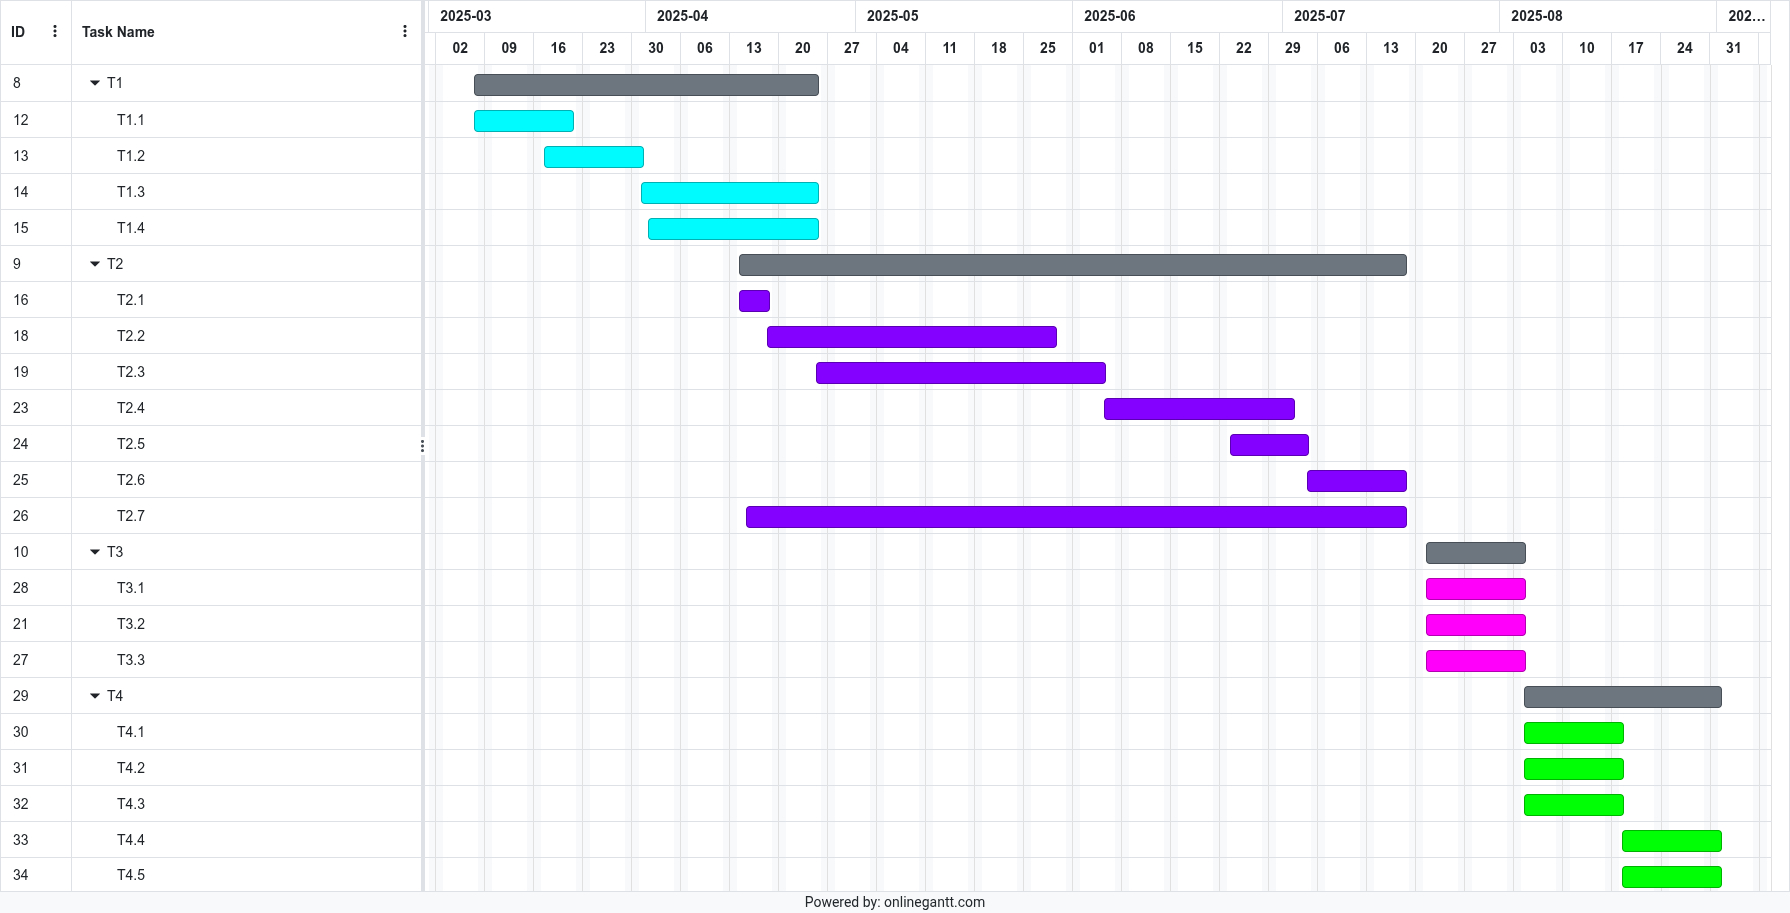
\includegraphics[width=\textwidth]{imagenes/cap2/diagrama_gantt.png}
    \caption{Diagrama de Gantt del proyecto}
    \label{fig:diagrama-gantt}
\end{figure}

\section{Estimación de costes}

A continuación, se detallan los recursos necesarios para llevar a cabo el proyecto, incluyendo hardware, software y recursos humanos, junto con una estimación de los costes asociados.

\textbf{Hardware}

\begin{itemize}
    \item Ordenador portátil LG Gram 14Z90Q-G.AA75B, este equipo se utilizará para el desarrollo general del trabajo: creación del código para las pruebas, gestión de las pruebas en el clustery creación de la memoria. Cuenta con un procesador Intel Core i7-1260P, 16 GB de RAM y 512 GB de almacenamiento SSD.

    \item Ordenador portátil Lenovo Legion 5, utilizado como plataforma principal para la ejecución de pruebas de rendimiento, especialmente aquellas que requieren aceleración por GPU. Este equipo está equipado con un procesador AMD Ryzen 7 4800H (8 núcleos y 16 hilos), 16 GB de memoria RAM DDR4, 512 GB de almacenamiento SSD NVMe y una tarjeta gráfica dedicada NVIDIA GeForce RTX 2060 con 6 GB de VRAM GDDR6. La presencia de la GPU NVIDIA permite la ejecución y evaluación de aplicaciones HPC que hacen uso de CUDA, así como la integración y validación del soporte de GPU en entornos contenerizados mediante NVIDIA Container Toolkit. Además, este equipo facilita la comparación de resultados entre ejecución nativa y contenerizada en escenarios reales de computación de alto rendimiento.

    \item Ordenador Apple Mac Mini M4, utilizado como plataforma de pruebas para la ejecución y validación de aplicaciones HPC en entornos macOS y arquitectura ARM. Este equipo incorpora un procesador Apple M4 con arquitectura ARM64, núcleos de alto rendimiento y eficiencia, GPU integrada de última generación y 16 GB de memoria unificada. El Mac Mini M4 permitirá evaluar la compatibilidad y el rendimiento de contenedores en sistemas Apple Silicon.
\end{itemize}

\textbf{Software}

\begin{itemize}
    \item Sistema operativo Ubuntu 24.04 LTS. Será la distribución Linux principal con la que vamos a trabajar, tanto en forma nativa, como en los contenedores.

    \item Sistema operativo Microsoft Windows 11 Home. Será la distribución con la que se ejecutarán las pruebas de compatibilidad y rendimiento en entornos Windows.

    \item Sistema operativo macOS Sequoia 15.5. Será la distribución con la que se ejecutarán las pruebas de compatibilidad y rendimiento en entornos Apple.
\end{itemize}

\textbf{Recursos humanos}.

\begin{table}[!ht]
    \centering
    \begin{tabular}{|l|l|r|}
        \hline
        \textbf{Dispositivo}   & \textbf{Descripción}             & \textbf{Coste (€)} \\
        \hline
        LG Gram 14Z90Q-G.AA75B & Portátil principal de desarrollo & 1\,200             \\
        Lenovo Legion 5        & Portátil de pruebas              & 1\,000             \\
        Apple Mac Mini M4      & Dispositivo de pruebas Apple     & 599                \\
        \hline
        \textbf{Total}         &                                  & \textbf{2\,799}    \\
        \hline
    \end{tabular}
    \caption{Costes estimados de hardware para el proyecto}
    \label{tab:costes-hardware}
\end{table}

En cuanto al software, los sistemas operativos Microsoft Windows 11 Home y macOS Sequoia 15.5 vienen incluidos en los dispositivos correspondientes, por lo que no se ha considerado un coste adicional. El sistema operativo Ubuntu 24.04 LTS es de código abierto y gratuito, por lo que tampoco se ha considerado un coste adicional.

\textbf{Recursos humanos}

En la tabla \ref{tab:recursos-humanos} se detalla el coste por hora, las horas estimadas y el coste total de los recursos humanos necesarios para llevar a cabo el proyecto.

\begin{table}[!ht]
    \centering
    \begin{tabular}{|l|l|r|r|r|}
        \hline
        \textbf{Recurso}        & \textbf{Puesto}  & \textbf{€/h} & \textbf{Horas} & \textbf{Total (€)} \\
        \hline
        Fernando Cuesta Bueno   & Desarrollador    & 20           & 260            & 5\,200             \\
        Juan José Escobar Pérez & Tutor/Supervisor & 50           & 50             & 2\,500             \\
        \hline
        \textbf{Total}          &                  &              &                & \textbf{7\,700}    \\
        \hline
    \end{tabular}
    \caption{Costes estimados de recursos humanos para el proyecto}
    \label{tab:recursos-humanos}
\end{table}

\textbf{Coste total del proyecto}

El coste total del proyecto se calcula sumando los costes de hardware, software y recursos humanos. En la tabla \ref{tab:coste-total} se detalla el coste total estimado.

\begin{table}[!ht]
    \centering
    \begin{tabular}{|l|r|}
        \hline
        \textbf{Concepto} & \textbf{Coste (€)} \\
        \hline
        Hardware          & 2\,799             \\
        Software          & 0                  \\
        Recursos humanos  & 7\,700             \\
        \hline
        \textbf{Total}    & \textbf{10\,499}   \\
        \hline
    \end{tabular}
    \caption{Coste total estimado del proyecto}
    \label{tab:coste-total}
\end{table}